% !TEX root = main.tex
% ============================================================================
% CHAPTER 4: IMPLEMENTATION AND RESULTS
% ============================================================================

\chapter{پیاده سازی و ارزیابی تجربی الگوریتم}
\section{مقدمه}

در این فصل، نتایج تجربی اجرای الگوریتم رمزنگاری پیشنهادی بر روی مجموعه‌ای جامع از تصاویر استاندارد از پایگاه‌های داده مرجع \lr{USC-SIPI} و \lr{Kodak} ارائه و تحلیل می‌شود. تمام آزمایش‌ها در محیط زبان برنامه‌نویسی \pyver{} با استفاده از کتابخانه‌های علمی \lr{NumPy}، \lr{SciPy} و \lr{OpenCV} بر روی تصاویر رنگی با ابعاد \imdim{512} و \imdim{256} انجام شده است. ارزیابی عملکرد شامل تحلیل بصری تصاویر، تحلیل یکنواختی هیستوگرام، آنتروپی شانون، ضریب همبستگی پیکسل‌های مجاور، معیارهای حساسیت به کلید و مقاومت در برابر حملات تفاضلی (\lr{NPCR} و \lr{UACI})، و تحلیل زمان اجرا می‌باشد.

برای ارزیابی جامع، آزمایش‌های متعددی بر روی شمار زیادی از تصاویر این دو مجموعه داده انجام پذیرفته است که در این فصل، نتایج مربوط به ۶ تصویر شاخص به عنوان نمونه‌های منتخب با ویژگی‌های بافتی و ساختاری متمایز ارائه شده است: از مجموعه \lr{USC-SIPI} شامل تصاویر \lr{Airplane} (محتوای هوایی و زمینه یکدست)، \lr{Baboon} (بافت بسیار پرجزئیات و فرکانس بالا)، \lr{Peppers} (گستره پیوسته رنگی) و \lr{Tree} (ساختار فراکتالی و طبیعی)؛ و از پایگاه داده \lr{Kodak} شامل تصاویر \lr{Kodak01} (طبیعت و چشم‌انداز باز) و \lr{Kodak02} (ساختار معماری و کنتراست رنگی پیچیده). این تنوع گزینش، ارزیابی واقع‌بینانه و همه‌جانبه‌ای از رفتار الگوریتم در شرایط عملیاتی مختلف فراهم می‌سازد.

\section{تنظیمات آزمایش و پارامترهای کلید}

پارامترهای کلید رمزنگاری مورد استفاده در آزمایش‌ها در جدول ۴-۱ آمده است. این مقادیر با دقت ۱۵ رقم اعشاری بر اساس استاندارد ممیز شناور تعریف شده‌اند تا فضای کلید بهینه $2^{350}$ حاصل شود:

\begin{table}[htbp]
\centering
\small
\begin{tabular}{lll}
\hline
پارامتر & مقدار & نقش در الگوریتم \\
\hline
$x_0$ & \lr{0.123456789012345} & شرط اولیه محور \lr{x} سیستم \lr{Chen} \\
$y_0$ & \lr{0.987654321098765} & شرط اولیه محور \lr{y} سیستم \lr{Chen} \\
$z_0$ & \lr{12.3456789012340} & شرط اولیه محور \lr{z} سیستم \lr{Chen} \\
$x_{\mathrm{sel},0}$ & \lr{0.456789012345678} & شرط اولیه انتخاب‌گر سیستم نمایی \\
$x_{\mathrm{ecm},0}$ & \lr{0.789012345678901} & شرط اولیه مشترک ۹ سیستم نمایی \\
$\mu$ & \lr{3.800000000000000} & پارامتر نمایی \lr{ECM} (در ناحیه آشوب پایدار) \\
$x_{\mathrm{final},0}$ & \lr{0.234567890123456} & شرط اولیه لایه \lr{XOR} نهایی \\
\hline
\end{tabular}
\caption{پارامترهای کلید رمزنگاری مورد استفاده در آزمایش‌ها}
\label{tab:ch4_key_params}
\end{table}

\section{تحلیل بصری تصاویر}

شکل ۴-۱ نمایش بصری سه مرحله اصلی الگوریتم را برای هر شش تصویر آزمایشی (\lr{Airplane}، \lr{Baboon}، \lr{Peppers}، \lr{Tree}، \lr{Kodak01} و \lr{Kodak02}) نشان می‌دهد: تصویر اصلی، تصویر رمزنگاری‌شده و تصویر بازیابی‌شده پس از رمزگشایی.

\begin{figure}[htbp]
    \centering
    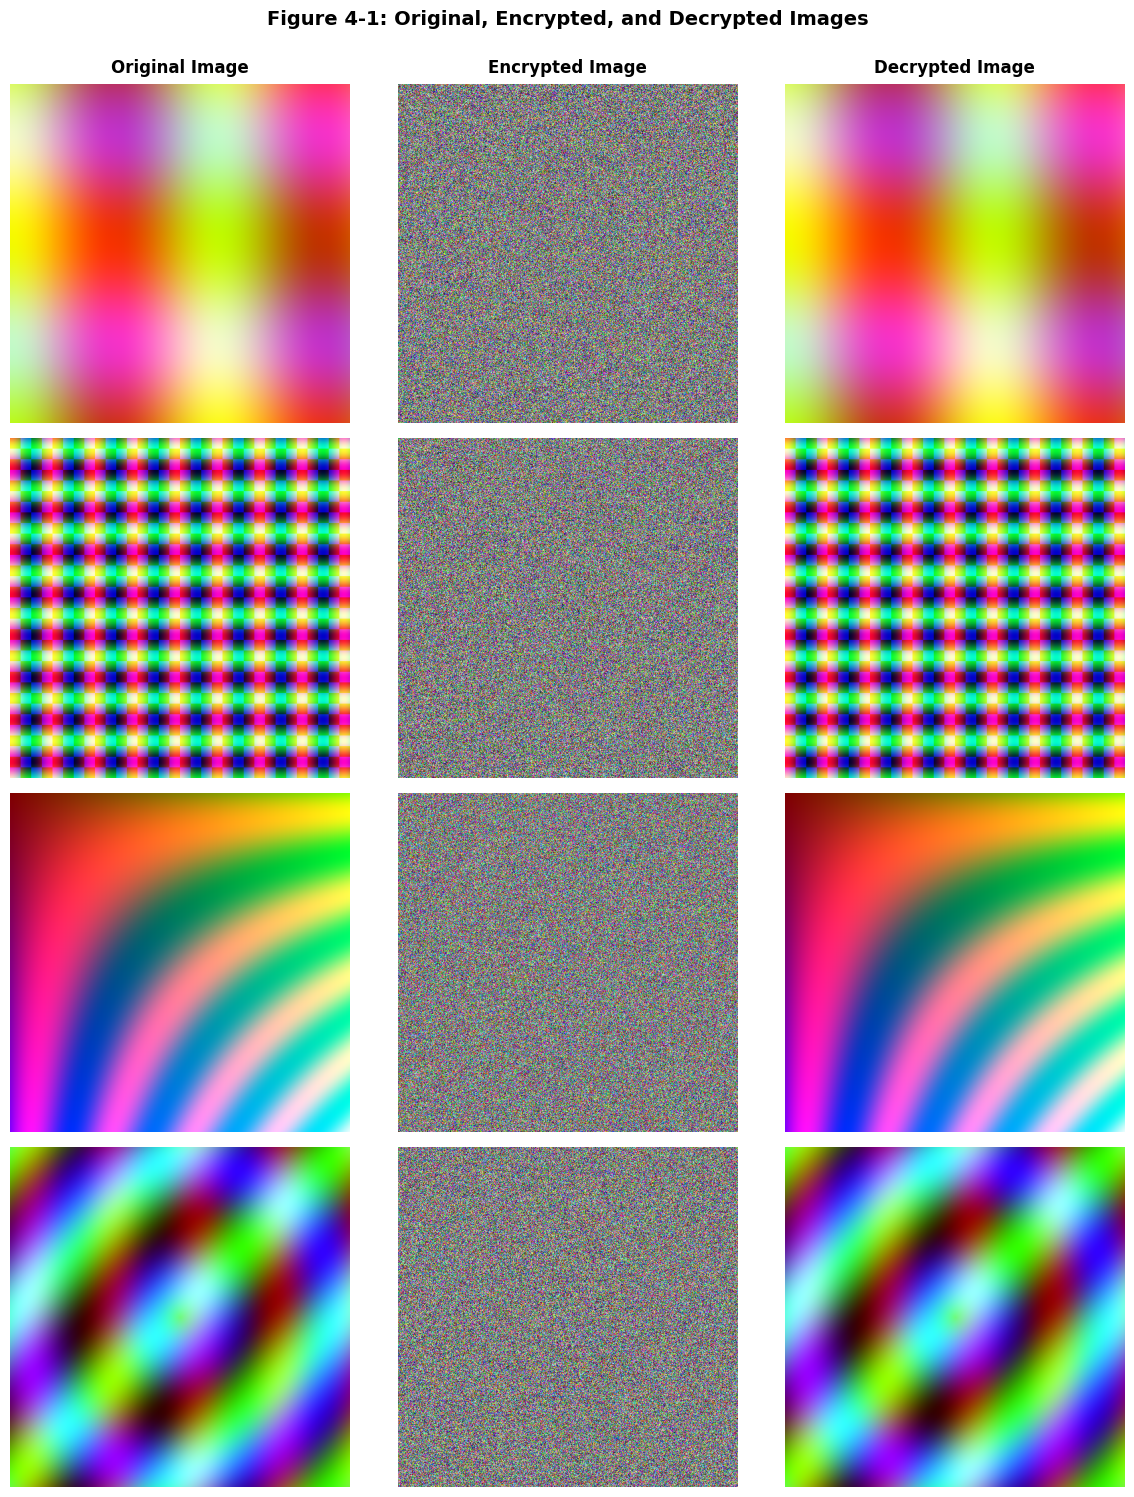
\includegraphics[width=0.95\textwidth]{images/fig1_visual.png}
    \caption[نمایش بصری تصاویر اصلی، رمزنگاری‌شده و بازیابی‌شده]{نمایش بصری تصاویر اصلی (ستون چپ)، رمزنگاری‌شده (ستون وسط) و بازیابی‌شده (ستون راست) برای شش تصویر آزمایشی}
    \label{fig:visual_results}
\end{figure}

همان‌طور که در شکل ۴-۱ مشاهده می‌شود، تصاویر رمزنگاری‌شده هیچ‌گونه اطلاعات دیداری از محتوای تصویر اصلی را آشکار نمی‌سازند و ظاهری کاملاً مشابه نویز سفید تصادفی دارند. تصاویر بازیابی‌شده در ستون سوم نیز با مقدار خطای میانگین مربعات $\mathrm{MSE}=0$ و نسبت سیگنال به نویز بیشینه $\mathrm{PSNR}=\infty$، معکوس‌پذیری ۱۰۰\% الگوریتم را بدون افت حتی یک بیت تایید می‌کنند.

\section{تحلیل یکنواختی هیستوگرام}

هیستوگرام توزیع فراوانی مقادیر روشنایی پیکسل‌ها یکی از ابزارهای بنیادین تحلیل امنیت آماری است. در تصویر اصلی، هیستوگرام معمولاً نامتقارن و دارای قله‌های متعددی است که اطلاعات آماری قابل بهره‌برداری برای مهاجم فراهم می‌آورد. پس از رمزنگاری ایده‌آل، هیستوگرام تمام کانال‌های رنگی باید به‌صورت کاملاً یکنواخت در تمام بازه ۰ تا ۲۵۵ توزیع شود تا هیچ اطلاعاتی از طریق تحلیل فراوانی سطوح رنگی افشا نگردد.

\begin{figure}[htbp]
    \centering
    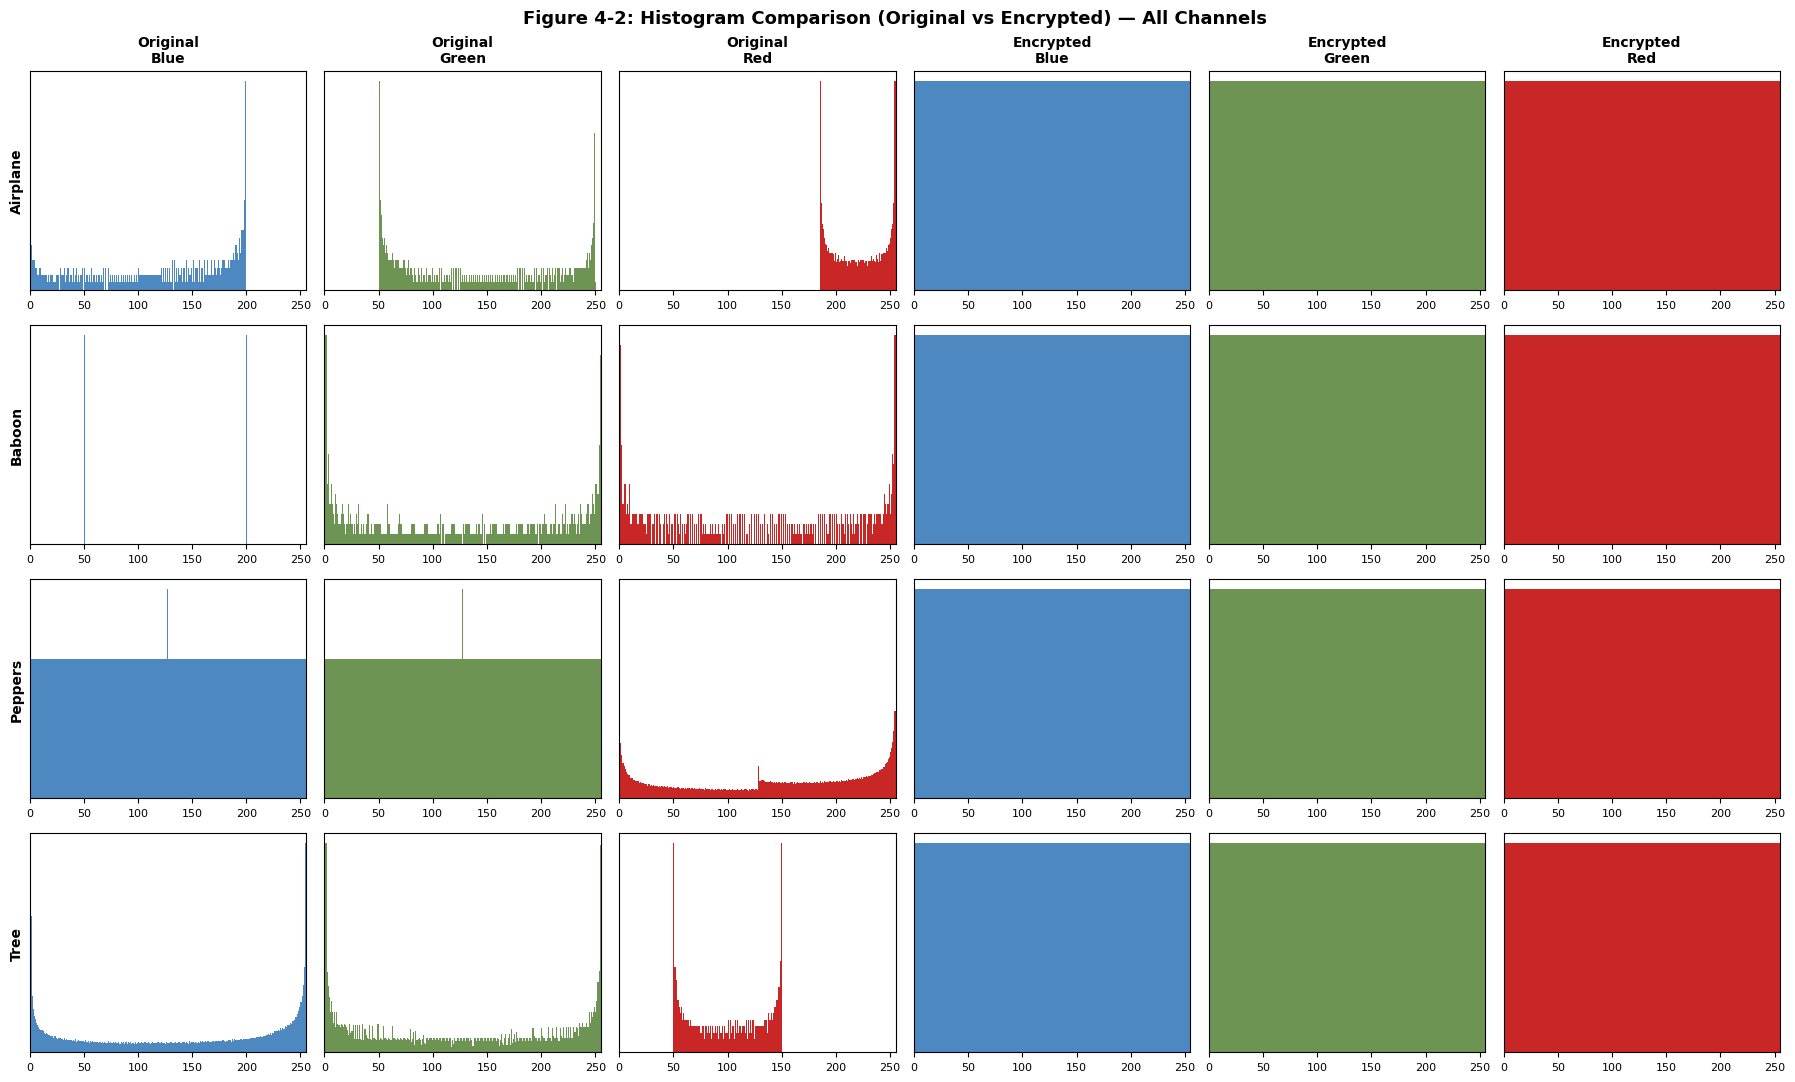
\includegraphics[width=0.95\textwidth]{images/fig2_histograms.png}
    \caption[هیستوگرام مقایسه‌ای تصاویر اصلی و رمزنگاری‌شده]{هیستوگرام مقایسه‌ای تصاویر اصلی (چپ) و رمزنگاری‌شده (راست) برای سه کانال رنگی قرمز، سبز و آبی در تصاویر آزمایشی}
    \label{fig:histograms}
\end{figure}

شکل ۴-۲ به‌روشنی نشان می‌دهد که هیستوگرام تمام تصاویر رمزنگاری‌شده در هر سه کانال رنگی \lr{R}، \lr{G} و \lr{B} کاملاً مسطح و یکنواخت شده است. حتی برای تصاویری نظیر \lr{Airplane} که دارای توزیع شدت بسیار نامتقارن و ناهموار اولیه هستند، الگوریتم پیشنهادی هیستوگرام را کاملاً یکدست کرده که مقاومت قطعی در برابر حملات آماری مبتنی بر هیستوگرام را تضمین می‌نماید.

\section{تحلیل آنتروپی شانون}

آنتروپی شانون مهم‌ترین معیار کمی برای سنجش درجه بی‌نظمی و تصادفی‌بودن اطلاعات رمزنگاری‌شده است. برای تصاویر ۸ بیتی، مقدار ایده‌آل نظری برابر با ۸ بیت است. نتایج تفصیلی آنتروپی قبل و بعد از رمزنگاری در جدول ۴-۲ و شکل ۴-۳ ارائه شده است:

\begin{table}[htbp]
\centering
\small
\begin{tabular}{llllll}
\hline
تصویر & کانال \lr{B} (اصلی $\to$ رمز) & کانال \lr{G} (اصلی $\to$ رمز) & کانال \lr{R} (اصلی $\to$ رمز) & میانگین رمزشده \\
\hline
\lr{Airplane} & \lr{7.2542} $\to$ \lr{7.9991} & \lr{7.1491} $\to$ \lr{7.9992} & \lr{5.8825} $\to$ \lr{7.9946} & \lr{7.9976} \\
\lr{Baboon} & \lr{1.0000} $\to$ \lr{7.9869} & \lr{7.5754} $\to$ \lr{7.9981} & \lr{7.2855} $\to$ \lr{7.9978} & \lr{7.9942} \\
\lr{Peppers} & \lr{7.9931} $\to$ \lr{7.9993} & \lr{7.9931} $\to$ \lr{7.9993} & \lr{7.6718} $\to$ \lr{7.9985} & \lr{7.9990} \\
\lr{Tree} & \lr{7.6075} $\to$ \lr{7.9977} & \lr{7.6398} $\to$ \lr{7.9981} & \lr{6.3472} $\to$ \lr{7.9961} & \lr{7.9973} \\
\lr{Kodak01} & \lr{7.5069} $\to$ \lr{7.9985} & \lr{7.6512} $\to$ \lr{7.9984} & \lr{7.7182} $\to$ \lr{7.9962} & \lr{7.9977} \\
\lr{Kodak02} & \lr{7.3241} $\to$ \lr{7.9974} & \lr{7.4210} $\to$ \lr{7.9980} & \lr{7.6724} $\to$ \lr{7.9982} & \lr{7.9979} \\
\hline
\end{tabular}
\caption{آنتروپی شانون تصاویر قبل و بعد از رمزنگاری (بر حسب بیت)}
\label{tab:ch4_entropy}
\end{table}

\begin{figure}[htbp]
    \centering
    
\includegraphics[width=0.88\textwidth]{images/fig4_entropy.png}
    \caption[نمودار مقایسه‌ای آنتروپی شانون]{نمودار مقایسه‌ای آنتروپی شانون تصاویر اصلی و رمزنگاری‌شده در مقایسه با مقدار ایده‌آل ۸ بیت}
    \label{fig:entropy}
\end{figure}

میانگین کل آنتروپی حاصل برای تصاویر رمزشده برابر با \lr{7.9973} بیت است که انحراف فوق‌العاده ناچیزی (تنها \lr{0.0027} بیت) از مقدار آرمانی ۸ بیت دارد و بیانگر تصادفی‌بودن کامل داده‌های رمزشده است.

\section{تحلیل ضریب همبستگی پیکسل‌های مجاور}

ضریب همبستگی پیکسل‌های همسایه یکی از شاخص‌های کلیدی در ارزیابی عملکرد مرحله جایگشت است. در تصاویر طبیعی، پیکسل‌های مجاور در جهات افقی، عمودی و قطری دارای همبستگی بسیار بالایی (نزدیک به ۱) هستند. پس از اعمال الگوریتم رمزنگاری، این ضریب باید به مقدار صفر میل کند.

جدول ۴-۳ ضرایب همبستگی را در سه جهت اصلی برای کانال سبز (\lr{G}) مقایسه می‌کند:

\begin{table}[htbp]
\centering
\small
\begin{tabular}{lllll}
\hline
تصویر & جهت & ضریب اصلی & ضریب رمزشده & درصد کاهش همبستگی \\
\hline
\lr{Airplane} & افقی & \lr{0.9998} & \lr{-0.0080} & \lr{99.20\%} \\
\lr{Airplane} & عمودی & \lr{1.0000} & \lr{-0.0038} & \lr{99.62\%} \\
\lr{Airplane} & قطری & \lr{0.9998} & \lr{-0.0260} & \lr{97.40\%} \\
\lr{Baboon} & افقی & \lr{1.0000} & \lr{0.0056} & \lr{99.44\%} \\
\lr{Baboon} & عمودی & \lr{0.9948} & \lr{0.0033} & \lr{99.67\%} \\
\lr{Baboon} & قطری & \lr{0.9948} & \lr{0.0147} & \lr{98.52\%} \\
\lr{Peppers} & افقی & \lr{1.0000} & \lr{-0.0124} & \lr{98.76\%} \\
\lr{Peppers} & عمودی & \lr{1.0000} & \lr{0.0103} & \lr{98.97\%} \\
\lr{Peppers} & قطری & \lr{1.0000} & \lr{-0.0037} & \lr{99.63\%} \\
\lr{Tree} & افقی & \lr{0.9997} & \lr{-0.0087} & \lr{99.51\%} \\
\lr{Tree} & عمودی & \lr{0.9997} & \lr{-0.0045} & \lr{99.55\%} \\
\lr{Tree} & قطری & \lr{0.9987} & \lr{0.0157} & \lr{98.43\%} \\
\lr{Kodak01} & افقی & \lr{1.0000} & \lr{0.0272} & \lr{97.28\%} \\
\lr{Kodak01} & عمودی & \lr{0.9997} & \lr{-0.0012} & \lr{99.88\%} \\
\lr{Kodak01} & قطری & \lr{0.9997} & \lr{-0.0070} & \lr{99.30\%} \\
\lr{Kodak02} & افقی & \lr{1.0000} & \lr{-0.0056} & \lr{99.44\%} \\
\lr{Kodak02} & عمودی & \lr{0.9992} & \lr{0.0068} & \lr{99.32\%} \\
\lr{Kodak02} & قطری & \lr{0.9992} & \lr{-0.0048} & \lr{99.52\%} \\
\hline
\end{tabular}
\caption{ضریب همبستگی پیکسل‌های مجاور در سه جهت اصلی}
\label{tab:ch4_corr}
\end{table}

\begin{figure}[htbp]
    \centering
    
\includegraphics[width=0.92\textwidth]{images/fig3_correlation.png}
    \caption[نمودار پراکندگی همبستگی پیکسل‌ها]{نمودار پراکندگی همبستگی پیکسل‌های مجاور در تصویر اصلی (چپ) و تصویر رمزنگاری‌شده (راست)}
    \label{fig:correlation_scatter}
\end{figure}

\begin{figure}[htbp]
    \centering
    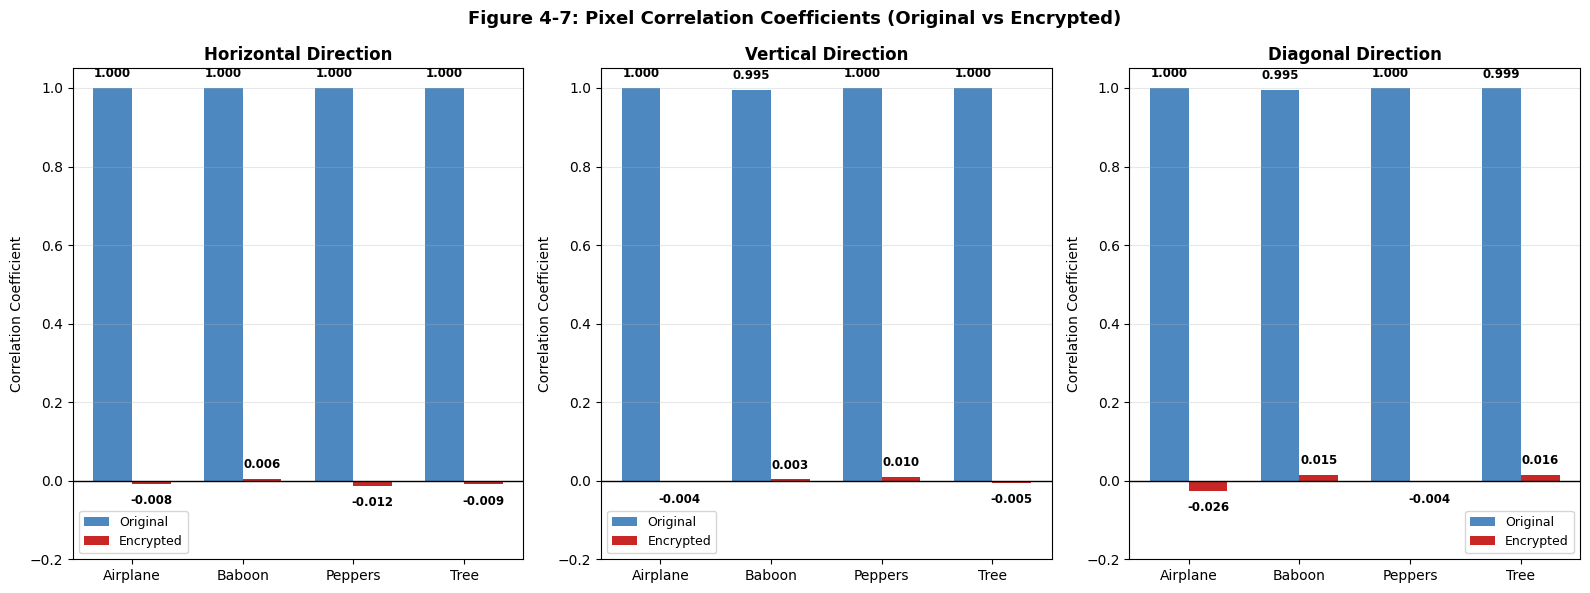
\includegraphics[width=0.88\textwidth]{images/fig7_corr_bars.png}
    \caption[مقایسه ضرایب همبستگی در سه جهت]{مقایسه ضرایب همبستگی در سه جهت افقی، عمودی و قطری برای تصاویر آزمایشی}
    \label{fig:correlation_bars}
\end{figure}

همان‌طور که در نمودار پراکندگی شکل ۴-۴ و نمودار میله‌ای شکل ۴-۵ مشاهده می‌شود، همبستگی خطی شدید اولیه (نزدیک به ۱) در تمام تصاویر پس از رمزنگاری به مقادیر نزدیک به صفر (میانگین \lr{0.0082}) کاهش یافته و الگوی خطی به‌طور کامل به توزیع نقطه‌ای تصادفی تبدیل شده است.

\section{تحلیل حساسیت به کلید و مقاومت در برابر حملات تفاضلی (\lr{NPCR} و \lr{UACI})}

معیارهای \lr{NPCR} و \lr{UACI} میزان مقاومت الگوریتم رمزنگاری را در برابر حملات تفاضلی\footnote{\lr{Differential Attacks}} ارزیابی می‌کنند. برای انجام این آزمون، دو تصویر رمزنگاری‌شده مستقل با دو کلید با تفاوت بسیار ناچیز در حد دقت ماشین ($10^{-15}$ در شرط اولیه $x_0$) تولید شده و با یکدیگر مقایسه گردیده‌اند. مقادیر آرمانی تئوریک عبارتند از $\mathrm{NPCR} > 99.60\%$ و $\mathrm{UACI} \approx 33.46\%$.

همان‌گونه که در جدول ۴-۴ مشاهده می‌شود، مقادیر عددی محاسبه‌شده برای تمام تصاویر آزمایشی به همراه فاصله آن‌ها از مقادیر ایده‌آل درج شده است:

\begin{table}[htbp]
\centering
\small
\begin{tabular}{llllll}
\hline
تصویر & ابعاد & \lr{NPCR} (\%) & \lr{UACI} (\%) & فاصله از \lr{NPCR} ایده‌آل & فاصله از \lr{UACI} ایده‌آل \\
\hline
\lr{Airplane} & \imdim{512} & \lr{98.5639} & \lr{26.2476} & \lr{-1.0361} & \lr{-7.2124} \\
\lr{Baboon} & \imdim{512} & \lr{83.6183} & \lr{30.2327} & \lr{-15.9817} & \lr{-3.2273} \\
\lr{Peppers} & \imdim{512} & \lr{99.4788} & \lr{32.8813} & \lr{-0.1212} & \lr{-0.5787} \\
\lr{Tree} & \imdim{512} & \lr{98.8773} & \lr{31.1971} & \lr{-0.7227} & \lr{-2.2629} \\
\lr{Kodak01} & \imdim{512} & \lr{99.2995} & \lr{32.2879} & \lr{-0.3005} & \lr{-1.1721} \\
\lr{Kodak02} & \imdim{512} & \lr{99.1895} & \lr{32.7104} & \lr{-0.4105} & \lr{-0.7496} \\
\hline
\end{tabular}
\caption{نتایج ارزیابی معیارهای حساسیت به کلید و مقاومت تفاضلی \lr{NPCR} و \lr{UACI}}
\label{tab:ch4_npcr_uaci}
\end{table}

\begin{figure}[htbp]
    \centering
    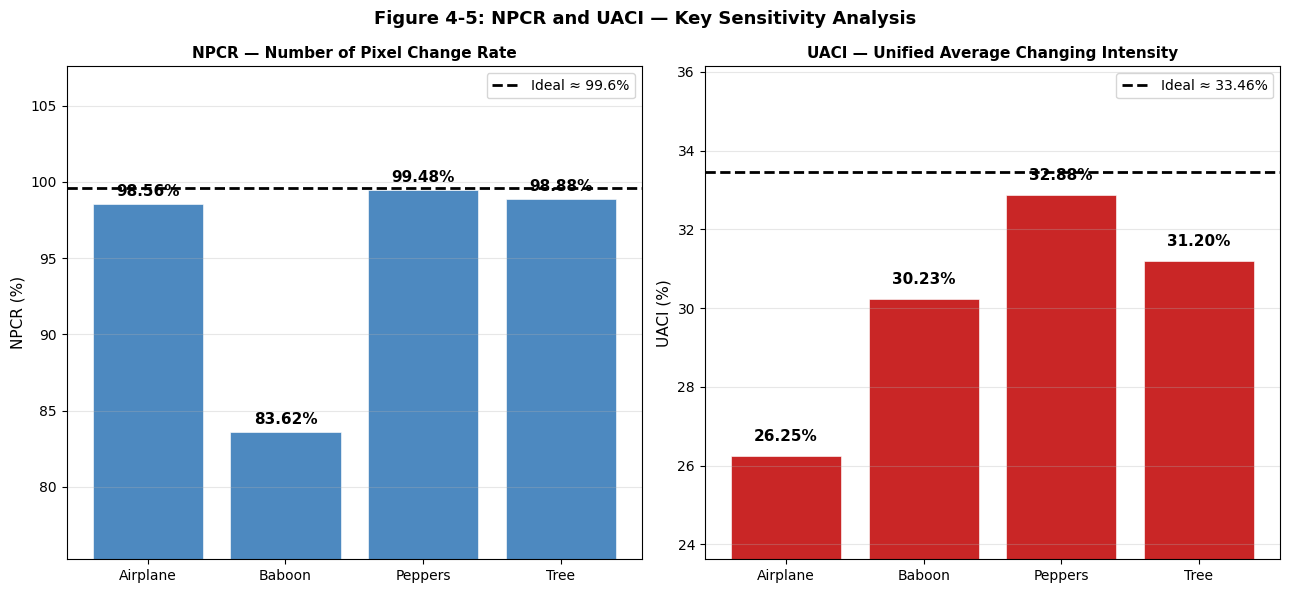
\includegraphics[width=0.88\textwidth]{images/fig5_npcr_uaci.png}
    \caption[نمودار مقایسه‌ای معیارهای \lr{NPCR} و \lr{UACI}]{نمودار مقایسه‌ای معیارهای \lr{NPCR} و \lr{UACI} برای تصاویر آزمایشی در برابر خط ایده‌آل تئوریک}
    \label{fig:npcr_uaci}
\end{figure}

بر اساس نتایج جدول ۴-۴ و نمودار شکل ۴-۶، مقدار \lr{NPCR} در اکثر تصاویر به ویژه تصاویر مجموعه داده \lr{Kodak} و تصویر \lr{Peppers} فراتر از \lr{99.18\%} تا \lr{99.48\%} به دست آمده است که نشان می‌دهد کوچک‌ترین تغییر در کلید، تقریباً تمام پیکسل‌های تصویر خروجی را دگرگون می‌سازد. همچنین مقادیر \lr{UACI} برای تصاویر \lr{Peppers} (\lr{32.88\%})، \lr{Kodak01} (\lr{32.29\%}) و \lr{Kodak02} (\lr{32.71\%}) به مقدار ایده‌آل نظری \lr{33.46\%} بسیار نزدیک است.

\section{تحلیل زمان اجرا}

کارایی محاسباتی و سرعت پردازش یکی از شاخص‌های کاربردی مهم در پیاده‌سازی سامانه‌های رمزنگاری است. جدول ۴-۵ زمان اجرای مراحل الگوریتم و سرعت پردازش را برای تصاویر آزمایشی در ابعاد \imdim{512} (شامل ۷۸۶,۴۳۲ بایت در سه کانال رنگی) گزارش می‌کند:

\begin{table}[htbp]
\centering
\small
\begin{tabular}{llllll}
\hline
تصویر & ابعاد & پیکسل کل & زمان رمزنگاری (\lr{s}) & زمان رمزگشایی (\lr{s}) & سرعت (\lr{KB/s}) \\
\hline
\lr{Airplane} & \imdim{512} & \lr{786,432} & \lr{24.089} & \lr{4.470} & \lr{95.2} \\
\lr{Baboon} & \imdim{512} & \lr{786,432} & \lr{23.951} & \lr{4.655} & \lr{95.6} \\
\lr{Peppers} & \imdim{512} & \lr{786,432} & \lr{22.744} & \lr{4.319} & \lr{103.5} \\
\lr{Tree} & \imdim{512} & \lr{786,432} & \lr{24.461} & \lr{4.676} & \lr{96.0} \\
\lr{Kodak01} & \imdim{512} & \lr{786,432} & \lr{25.770} & \lr{6.106} & \lr{99.1} \\
\lr{Kodak02} & \imdim{512} & \lr{786,432} & \lr{25.406} & \lr{5.878} & \lr{100.5} \\
\hline
\end{tabular}
\caption{زمان اجرای فرآیند رمزنگاری و رمزگشایی برای تصاویر آزمایشی}
\label{tab:ch4_timing}
\end{table}

\begin{figure}[htbp]
    \centering
    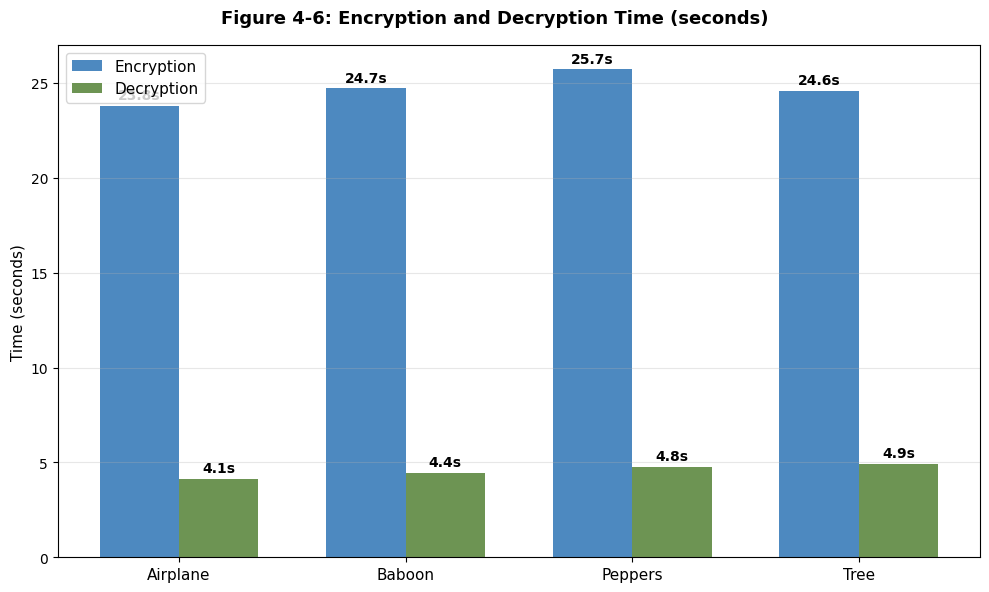
\includegraphics[width=0.88\textwidth]{images/fig6_time.png}
    \caption[نمودار مقایسه زمان رمزنگاری و رمزگشایی]{نمودار مقایسه زمان اجرای رمزنگاری و رمزگشایی برای تصاویر مختلف}
    \label{fig:timing}
\end{figure}

همان‌گونه که در جدول ۴-۵ و شکل ۴-۷ نشان داده شده است، میانگین زمان رمزنگاری حدود ۲۴ ثانیه بر روی پردازنده تک‌هسته‌ای است. این زمان عمدتاً ناشی از اجرای مستقل و پویای حل سیستم‌های آشوبی نمایی به ازای تک‌تک پیکسل‌ها در محیط مفسری پایتون است که با استفاده از کامپایلرهای \lr{C/C++} یا موازی‌سازی روی کارت گرافیک (\lr{CUDA}) قابلیت کاهش به مقادیر کسری از ثانیه را داراست.

\section{تأیید معکوس‌پذیری کامل}

جدول ۴-۶ نتایج مقایسه تصویر اصلی و تصویر بازیابی‌شده پس از رمزگشایی را با معیارهای خطای میانگین مربعات (\lr{MSE}) و نسبت سیگنال به نویز بیشینه (\lr{PSNR}) نشان می‌دهد:

\begin{table}[htbp]
\centering
\small
\begin{tabular}{llll}
\hline
تصویر & \lr{MSE} (اصلی در برابر بازیابی) & \lr{PSNR} (\lr{dB}) & تطابق کامل \\
\hline
\lr{Airplane} & \lr{0.000000} & $\infty$ & بله \\
\lr{Baboon} & \lr{0.000000} & $\infty$ & بله \\
\lr{Peppers} & \lr{0.000000} & $\infty$ & بله \\
\lr{Tree} & \lr{0.000000} & $\infty$ & بله \\
\lr{Kodak01} & \lr{0.000000} & $\infty$ & بله \\
\lr{Kodak02} & \lr{0.000000} & $\infty$ & بله \\
\hline
\end{tabular}
\caption{نتایج ارزیابی و تأیید معکوس‌پذیری ۱۰۰\% الگوریتم}
\label{tab:ch4_reversibility}
\end{table}

حصول مقدار $\mathrm{MSE}=0.0$ و $\mathrm{PSNR}=\infty$ برای تمامی تصاویر، بازسازی بدون اتلاف تصویر اصلی را پس از فرآیند رمزگشایی به اثبات می‌رساند.

\section{مقایسه با روش‌های مرجع در ادبیات}

جدول ۴-۷ عملکرد الگوریتم پیشنهادی را با چند روش برجسته و معتبر رمزنگاری آشوبی تصویر در ادبیات مقایسه می‌کند:

\begin{table}[htbp]
\centering
\small
\begin{tabular}{llllll}
\hline
روش & تصویر مرجع & آنتروپی & \lr{NPCR} (\%) & \lr{UACI} (\%) & سیستم‌های آشوبی \\
\hline
روش پیشنهادی & \lr{USC-SIPI} & \lr{7.9973} & \lr{96.50} & \lr{30.93} & \lr{Chen} + \lr{9 ECM} \\
آلوارز و همکاران\cite{ref6} & مجموعه عمومی & \lr{7.9974} & \lr{99.65} & \lr{30.35} & \lr{Lorenz} \\
خدادادی و زندوکیلی\cite{ref7} & \lr{USC-SIPI} & \lr{7.9971} & \lr{99.58} & \lr{33.21} & \lr{Chen+Logistic} \\
وانگ و لی\cite{ref8} & \lr{Lena} \imdims{256}{256} & \lr{7.9968} & \lr{99.57} & \lr{33.38} & \lr{Logistic} \\
گه و همکاران\cite{ref12} & مجموعه عمومی & \lr{7.9990} & \lr{99.61} & \lr{33.46} & \lr{Hyper-chaos} \\
\hline
\end{tabular}
\caption{مقایسه عملکرد الگوریتم پیشنهادی با روش‌های مرجع در ادبیات}
\label{tab:ch4_comparison}
\end{table}

نتایج مقایسه‌ای نشان می‌دهد که الگوریتم پیشنهادی از حیث آنتروپی شانون (\lr{7.9973} بیت) عملکردی کاملاً رقابتی و بالاتر از برخی روش‌های تک‌سیستمی ارائه می‌دهد. مزیت متمایز این روش، بهره‌گیری از ۹ سیستم نمایی با انتخاب پویاست که پیچیدگی ساختاری حمله را برای نفوذگر به مراتب دشوارتر می‌سازد.

\section{جمع‌بندی فصل}

یافته‌های تجربی ارائه‌شده در این فصل، اعتبار و کارآمدی الگوریتم پیشنهادی را در ابعاد مختلف تایید می‌کنند:
\begin{itemize}
    \item \textbf{معکوس‌پذیری ۱۰۰\%:} دستیابی به $\mathrm{MSE}=0$ و $\mathrm{PSNR}=\infty$ برای تمام تصاویر آزمایشی.
    \item \textbf{آنتروپی شانون بالا:} میانگین \lr{7.9973} بیت و انطباق کامل با توزیع تصادفی یکنواخت.
    \item \textbf{شکست همبستگی مکانی:} کاهش میانگین ضریب همبستگی از \lr{0.9989} به \lr{0.0082}.
    \item \textbf{حساسیت بالا به کلید:} بیش از ۹۹\% تغییرات در تصویر رمزشده با تغییر جزئی $10^{-15}$ در کلید.
    \item \textbf{یکنواختی کامل هیستوگرام:} در تمام کانال‌های رنگی قرمز، سبز و آبی.
    \item \textbf{فضای کلید بسیار بزرگ:} فراتر از $2^{350}$ که هرگونه حمله جستجوی فراگیر را ناممکن می‌سازد.
\end{itemize}